\documentclass{article}
% ~ ~ ~ ~ ~ ~ ~ ~ ~ ~ ~ ~ ~ ~ ~ ~ ~ ~ ~ ~ ~ ~ ~ ~ ~ ~ ~ ~ ~ ~ ~ ~ ~ ~ ~ ~ ~ ~ ~ ~ ~ ~ ~ ~ ~ ~ ~ ~

\usepackage[utf8]{inputenc}
\usepackage{amsmath}
\usepackage{amssymb} % for \mathbb
\usepackage{graphicx} % for figures
\usepackage{color}
\usepackage[usenames,dvipsnames]{xcolor}
\usepackage{hyperref} % for hyperlinks
\usepackage{float} % for figures
% ~ ~ ~ ~ ~ ~ ~ ~ ~ ~ ~ ~ ~ ~ ~ ~ ~ ~ ~ ~ ~ ~ ~ ~ ~ ~ ~ ~ ~ ~ ~ ~ ~ ~ ~ ~ ~ ~ ~ ~ ~ ~ ~ ~ ~ ~ ~ ~
% CUSTOM COLOUR
\definecolor{DGrey}{rgb}{0.1,0.1,0.1} % Dark Grey
% ~ ~ ~ ~ ~ ~ ~ ~ ~ ~ ~ ~ ~ ~ ~ ~ ~ ~ ~ ~ ~ ~ ~ ~ ~ ~ ~ ~ ~ ~ ~ ~ ~ ~ ~ ~ ~ ~ ~ ~ ~ ~ ~ ~ ~ ~ ~ ~
\title{ Introduction to Engineering Written Assignment Questions}
\date{January 2013}
\author{Greg Mayer and Daniel Connelly}
% ~ ~ ~ ~ ~ ~ ~ ~ ~ ~ ~ ~ ~ ~ ~ ~ ~ ~ ~ ~ ~ ~ ~ ~ ~ ~ ~ ~ ~ ~ ~ ~ ~ ~ ~ ~ ~ ~ ~ ~ ~ ~ ~ ~ ~ ~ ~ ~
% HEADER/FOOTER
\usepackage{fancyheadings}
\pagestyle{myheadings} % set headings to be user defined
\fancyhead{} % To create custom header, clear default layout
\renewcommand{\subsectionmark}[1]{\markright{{\color{DGrey}\thesubsection} \ {\color{DGrey}#1}}}
\fancyhead[LE,LO]{\subsectionmark} % To create custom header, clear default layout

% ~ ~ ~ ~ ~ ~ ~ ~ ~ ~ ~ ~ ~ ~ ~ ~ ~ ~ ~ ~ ~ ~ ~ ~ ~ ~ ~ ~ ~ ~ ~ ~ ~ ~ ~ ~ ~ ~ ~ ~ ~ ~ ~ ~ ~ ~ ~ ~
% ENUMERATION

\usepackage{enumitem}   % so that question numbers can be formatted 
\setenumerate[1]{label=\thesubsection.\arabic*.} % enumerate environment: add section numbers to items
% ~ ~ ~ ~ ~ ~ ~ ~ ~ ~ ~ ~ ~ ~ ~ ~ ~ ~ ~ ~ ~ ~ ~ ~ ~ ~ ~ ~ ~ ~ ~ ~ ~ ~ ~ ~ ~ ~ ~ ~ ~ ~ ~ ~ ~ ~ ~ ~
% MARGINS
\usepackage{anysize}
\marginsize{2.5cm}{2.5cm}{1cm}{1cm}
% ~ ~ ~ ~ ~ ~ ~ ~ ~ ~ ~ ~ ~ ~ ~ ~ ~ ~ ~ ~ ~ ~ ~ ~ ~ ~ ~ ~ ~ ~ ~ ~ ~ ~ ~ ~ ~ ~ ~ ~ ~ ~ ~ ~ ~ ~ ~ ~
% PAGE NUMBERING
\pagenumbering{arabic}
% ~ ~ ~ ~ ~ ~ ~ ~ ~ ~ ~ ~ ~ ~ ~ ~ ~ ~ ~ ~ ~ ~ ~ ~ ~ ~ ~ ~ ~ ~ ~ ~ ~ ~ ~ ~ ~ ~ ~ ~ ~ ~ ~ ~ ~ ~ ~ ~
% Custom Commands
\newcommand{\Emph}[1]{\textbf{#1}} % Emphasize
\newcommand{\R}{\mathbb{R}} 
\newcommand{\BM}{\begin{bmatrix}} % Begin Matrix
\newcommand{\EM}{\end{bmatrix}} % End Matrix
\newcommand{\BEN}{\begin{enumerate}[leftmargin=1.1cm]}% Begin ENumerate
\newcommand{\EEN}{\end{enumerate}} % End ENumerate
\newcommand{\MB}{\mathbf} % Math Bold

\newcommand{\px}{\frac{\partial}{\partial x}} % Partial wrt x
\newcommand{\py}{\frac{\partial}{\partial y}} % Partial wrt y

\newcommand{\pfx}{\frac{\partial f}{\partial x}} % Partial of f wrt x
\newcommand{\pfy}{\frac{\partial f}{\partial y}} % Partial of f wrt y
\newcommand{\pfxy}{\frac{\partial^2 f}{\partial y \partial x}} % Partial of f wrt y
\newcommand{\pfyx}{\frac{\partial^2 f}{\partial x \partial y}} % Partial of f wrt y

\newcommand{\ux}{\frac{\partial u}{\partial x }} % Partial of u wrt x
\newcommand{\uk}{\frac{\partial u}{\partial k }} % Partial of u wrt k
\newcommand{\ut}{\frac{\partial u}{\partial t}} % Partial of u wrt t
\newcommand{\utt}{\frac{\partial^2u}{\partial t^2}} % Partial of u wrt t
\newcommand{\us}{\frac{\partial u}{\partial s}} % Partial of u wrt t
\newcommand{\uss}{\frac{\partial^2 u}{\partial s^2}} % Partial of u wrt t
\newcommand{\kx}{\frac{\partial k}{\partial x }} % Partial of k wrt x
\newcommand{\kt}{\frac{\partial k}{\partial t }} % Partial of k wrt t

\newcommand{\pxu}{\frac{\partial x}{\partial u}} % x wrt u
\newcommand{\pxv}{\frac{\partial x}{\partial v}} % x wrt v
\newcommand{\pxw}{\frac{\partial x}{\partial w}} % x wrt v
\newcommand{\pxt}{\frac{\partial x}{\partial t}} % x wrt t
\newcommand{\pyu}{\frac{\partial y}{\partial u}} % y wrt u
\newcommand{\pyv}{\frac{\partial y}{\partial v}} % y wrt v
\newcommand{\pyw}{\frac{\partial y}{\partial w}} % y wrt v
\newcommand{\pyt}{\frac{\partial y}{\partial t}} % y wrt t
\newcommand{\pzu}{\frac{\partial z}{\partial u}} % z wrt u
\newcommand{\pzv}{\frac{\partial z}{\partial v}} % z wrt v
\newcommand{\pzw}{\frac{\partial z}{\partial w}} % z wrt v
\newcommand{\pzt}{\frac{\partial z}{\partial t}} % z wrt t


\newcommand{\VCT}{\textit{Vector Calculus} by Michael Corral} % Vector Calculus Textbook
\newcommand{\CAT}{\textit{College Algebra} by Carl Stitz and Jeff Zeager} % College Algebra Textbook
\newcommand{\From}{The following questions are related to } % Questions ....
% ~ ~ ~ ~ ~ ~ ~ ~ ~ ~ ~ ~ ~ ~ ~ ~ ~ ~ ~ ~ ~ ~ ~ ~ ~ ~ ~ ~ ~ ~ ~ ~ ~ ~ ~ ~ ~ ~ ~ ~ ~ ~ ~ ~ ~ ~ ~ ~
% ONLY USED FOR EDITING
\newcommand{\rednote}[1]{{\color{red}\textit{\textbf{#1}}}} % Shortcut for formatting notes for developers
\newcommand{\FromC}[1]{{\color{DGrey}\textit{#1}}} % Shortcut for coloring the "from" text
% ~ ~ ~ ~ ~ ~ ~ ~ ~ ~ ~ ~ ~ ~ ~ ~ ~ ~ ~ ~ ~ ~ ~ ~ ~ ~ ~ ~ ~ ~ ~ ~ ~ ~ ~ ~ ~ ~ ~ ~ ~ ~ ~ ~ ~ ~ ~ ~
% AUGMENTED MATRIX MACRO
% thanks to http://tex.stackexchange.com/questions/2233/whats-the-best-way-make-an-augmented-coefficient-matrix
\newenvironment{amatrix}[1]{%
  \left[\begin{array}{@{}*{#1}{c}|c@{}}
}{%
  \end{array}\right]
}
% ~ ~ ~ ~ ~ ~ ~ ~ ~ ~ ~ ~ ~ ~ ~ ~ ~ ~ ~ ~ ~ ~ ~ ~ ~ ~ ~ ~ ~ ~ ~ ~ ~ ~ ~ ~ ~ ~ ~ ~ ~ ~ ~ ~ ~ ~ ~ ~
% PAGE LAYOUT
\addtolength{\topmargin}{10pt}
\addtolength{\headsep}{10pt}
\addtolength{\textheight}{-20pt}



\setenumerate[1]{label=\arabic*.} % enumerate environment: add section numbers to items

%\usepackage{multienum}
%\usepackage{wrapfig}

\date{}
% ~ ~ ~ ~ ~ ~ ~ ~ ~ ~ ~ ~ ~ ~ ~ ~ ~ ~ ~ ~ ~ ~ ~ ~ ~ ~ ~ ~ ~ ~ ~ ~ ~ ~ ~ ~ ~ ~ ~ ~ ~ ~ ~ ~ ~ ~ ~ ~
\begin{document}
\begin{center}
\textsc{\LARGE Midterm 2}\\[0.5cm]
\end{center}
\section*{Questions}

\begin{enumerate}
\item % EVEN AND ODD
Determine the value of
\begin{align*}
  \mathop{\int_0^{\pi} \!\! \int_{-1}^1} x^4e^{x^2 + y^2}\sin(y) dydx.
\end{align*}
Do not use integration by parts, and do not use a change of variables. 
% ~~~~~~~~~~~~~~~~~~~~~~~~~~~~~~~~~~~~~~~~~~~~~~~~~~~~~~~~~~~~~~~~~~~~~~~~~~~~~~~~~


% ~~~~~~~~~~~~~~~~~~~~~~~~~~~~~~~~~~~~~~~~~~~~~~~~~~~~~~~~~~~~~~~~~~~~~~~~~~~~~~~~~
\item % CHANGING ORDER OF INTEGRATION
The volume, $V$, of the solid bounded by
\begin{align*}
  z=0, \quad x=y^2, \quad x+z=1
\end{align*}
can be found using the triple integral 
\begin{align*}
  V = \mathop{\int_{0}^{1} \!\! \int_{-\sqrt{x}}^{\sqrt{x}} \! \int_0^{1-x} } dz\ dy\ dx = \frac{8}{15}.
\end{align*}
By simply changing the order of integration, we can find five other ways of expressing the volume of the solid. Find three of them. 

Note that for this question, you do not need to perform any integration. Simply set up three other triple integrals that represent the volume of the solid.
\textit{Hint: you may however want to check that your integrals represent the same volume with WolframAlpha}.
% ~~~~~~~~~~~~~~~~~~~~~~~~~~~~~~~~~~~~~~~~~~~~~~~~~~~~~~~~~~~~~~~~~~~~~~~~~~~~~~~~~
\item % TRIG OPTIMIZATION
Show that 
\begin{align*}
  \sin\frac{a}{2} \ \sin\frac{b}{2} \ \sin\frac{c}{2}\le\frac{1}{8}.
\end{align*}
% ~~~~~~~~~~~~~~~~~~~~~~~~~~~~~~~~~~~~~~~~~~~~~~~~~~~~~~~~~~~~~~~~~~~~~~~~~~~~~~~~~
\item % TEMPERATURE
The temperature of the wire $x^2+y^2\le1$ in $\R^3$ is $T(x,y)=xy$. Find the coldest and hottest points or regions of the wire. 
% ~~~~~~~~~~~~~~~~~~~~~~~~~~~~~~~~~~~~~~~~~~~~~~~~~~~~~~~~~~~~~~~~~~~~~~~~~~~~~~~~~
\item % FUNNY AREA
It can be shown that 
\begin{align*}
  \int_0^a e^{-x^2}dx 
\end{align*}
exists, but cannot be expressed in terms of elementary functions\footnote{An elementary function is a function that is constructed from any finite combination of exponential, logarithmic, polynomial, root, and trigonometric functions.}. A two dimensional analogue of this integral is
\begin{align*}
  \iint_D e^{-x^2-y^2} dA,
\end{align*}
where $D$ is the disk $x^2+y^2\le a^2$. Are you able to determine the value of this integral using the techniques covered in this course? If so, what is this integral equal to? If not, explain why. 

% ~~~~~~~~~~~~~~~~~~~~~~~~~~~~~~~~~~~~~~~~~~~~~~~~~~~~~~~~~~~~~~~~~~~~~~~~~~~~~~~~~
\item % WHEN LAGRANGE DOESN'T WORK
This question has two parts.
\BEN
\item Find the minimum value of $f(x,y) = y$, subject to the constraint $64x^2-y^3=0$, using any method you like.
\item Show that the method of Lagrange Multipliers does not work for the problem in part (a). 
\EEN
% ~~~~~~~~~~~~~~~~~~~~~~~~~~~~~~~~~~~~~~~~~~~~~~~~~~~~~~~~~~~~~~~~~~~~~~~~~~~~~~~~~
\item % SIMPLE CHAIN RULE
Let $f=f(x,y)$ and $g=g(t)=f(\sin t, e^t+\cos t)$. Find an expression for $g'(t)$.
% ~~~~~~~~~~~~~~~~~~~~~~~~~~~~~~~~~~~~~~~~~~~~~~~~~~~~~~~~~~~~~~~~~~~~~~~~~~~~~~~~~
\item % WAVE EQUATION
If $f=f(t)$ and $g=g(t)$ are functions of one variable whose second derivatives exist, and \\ $u=f(s+ct)+g(s-ct)$, show that 
\begin{align*}
  \utt=c^2\uss,
\end{align*}
where $c$ is a constant. 
% ~~~~~~~~~~~~~~~~~~~~~~~~~~~~~~~~~~~~~~~~~~~~~~~~~~~~~~~~~~~~~~~~~~~~~~~~~~~~~~~~~
\item % CYLINDERS VOLUME
Find the volume bounded by the cylinders $x^2+y^2=1$ and $x^2+y^2 = 4$, and bounded by \\ $z = \ln(x^2+y^2)$. You may use the formula $\int \ln(x)dx = x\ln(x)-x+C$. 
% ~~~~~~~~~~~~~~~~~~~~~~~~~~~~~~~~~~~~~~~~~~~~~~~~~~~~~~~~~~~~~~~~~~~~~~~~~~~~~~~~~
\item % FUNCTION THAT IS NOT A GRADIENT
Let $f(x,y)$ be a function of two variables that has the form $f(x,y) = g_1(x,y)\MB{i} + g_2(x,y)\MB{j}$.
\BEN
\item Provide an example of an $f(x,y)$ that has the form $f(x,y) = g_1(x,y)\MB{i} + g_2(x,y)\MB{j}$, and has the property that there does not exist an $F(x,y)$ such that $\nabla F = f(x,y)$. 
\item Show that, for the function you chose in part (a), that there does not exist an $F$ such that $\nabla F=f$.
\EEN

% ~~~~~~~~~~~~~~~~~~~~~~~~~~~~~~~~~~~~~~~~~~~~~~~~~~~~~~~~~~~~~~~~~~~~~~~~~~~~~~~~~
\end{enumerate} % END OF QUESTIONS
% ~~~~~~~~~~~~~~~~~~~~~~~~~~~~~~~~~~~~~~~~~~~~~~~~~~~~~~~~~~~~~~~~~~~~~~~~~~~~~~~~~
% ~~~~~~~~~~~~~~~~~~~~~~~~~~~~~~~~~~~~~~~~~~~~~~~~~~~~~~~~~~~~~~~~~~~~~~~~~~~~~~~~~
% SOLUTIONS
\newpage
\section*{Solutions}

\begin{enumerate}
% ~~~~~~~~~~~~~~~~~~~~~~~~~~~~~~~~~~~~~~~~~~~~~~~~~~~~~~~~~~~~~~~~~~~~~~~~~~~~~~~~~
\item % EVEN AND ODD
The integral can be written as
\begin{align*}
  \mathop{\int_0^{\pi} \!\! \int_{-1}^1} e^{x^2 + y^2}\sin(y) dydx 
  &= \mathop{\int_0^{\pi} \!\! \int_{-1}^1} e^{x^2}e^{y^2}\sin(y) dydx  = \Bigg( \int_0^{\pi} e^{x^2} dx \Bigg)\Bigg( \int_{-1}^1 e^{y^2}\sin(y)dy \Bigg)  
\end{align*}
The second term is the integral of an odd function over a symmetrical interval, and so is equal to zero. Therefore,
\begin{align*}
  \mathop{\int_0^{\pi} \!\! \int_{-1}^1} e^{x^2 + y^2}\sin(y) dydx =0.
\end{align*}

% ~~~~~~~~~~~~~~~~~~~~~~~~~~~~~~~~~~~~~~~~~~~~~~~~~~~~~~~~~~~~~~~~~~~~~~~~~~~~~~~~~

% ~~~~~~~~~~~~~~~~~~~~~~~~~~~~~~~~~~~~~~~~~~~~~~~~~~~~~~~~~~~~~~~~~~~~~~~~~~~~~~~~~
\item % CHANGING ORDER OF INTEGRATION
Noting that the limits of integration are not dependent on $y$, the $z$ and the $y$ integrals can be interchanged:
\begin{align*}
  V &= \mathop{\int_{0}^{1} \!\! \int_{-\sqrt{x}}^{\sqrt{x}} \! \int_0^{1-x} } dz\ dy\ dx \\
   &= \mathop{\int_{0}^{1} \Bigg( \int_{-\sqrt{x}}^{\sqrt{x}} dy \Bigg) \Bigg( \int_0^{1-x} } dz\Bigg) dx \\
   &= \mathop{\int_{0}^{1}  \Bigg( \int_0^{1-x} } dz\Bigg) \Bigg( \int_{-\sqrt{x}}^{\sqrt{x}} dy \Bigg)dx \\
   &= \mathop{\int_{0}^{1} \!\! \int_0^{1-x} \!\! \int_{-\sqrt{x}}^{\sqrt{x}}} dy\ dz\ dx 
\end{align*}
We can also integrate $y$ last. We are given that the solid can be expressed as the region 
\begin{align*}
  S = \{(x,y,z)\ |\  0 \le x \le 1, -\sqrt{x} \le y \le \sqrt{x}, 0 \le z \le 1-x \}.
\end{align*}
We can re-write this as
\begin{align*}
  S = \{(x,y,z)\ |\  y^2 \le x \le 1, -1 \le y \le 1, 0 \le z \le 1-x \}.
\end{align*}
This gives us the integral
\begin{align*}
  V &= \mathop{\int_{-1}^{1} \! \int_{y^2}^{1} \! \int_0^{1-x} } dz\ dx\ dy
\end{align*}
We can also define the region in this way \rednote{wrong}
\begin{align*}
  S = \{(x,y,z)\ |\  0 \le x \le 1-z, -1 \le y \le 1, 0 \le z \le 1 \}.
\end{align*}
This gives us the integral
\begin{align*}
  V &= \mathop{\int_{-1}^{1} \! \int_{0}^{1} \! \int_0^{1-z} } dx\ dz\ dy
\end{align*}
% ~~~~~~~~~~~~~~~~~~~~~~~~~~~~~~~~~~~~~~~~~~~~~~~~~~~~~~~~~~~~~~~~~~~~~~~~~~~~~~~~~
\item % TRIG OPTIMIZATION
Let $f$ be
\begin{align*}
  f(a,b,c) &=  \sin\frac{a}{2} \ \sin\frac{b}{2} \ \sin\frac{c}{2}
\end{align*}
Then,
\begin{align*}
  \frac{\partial f}{\partial a} &=  \frac{1}{2}\cos\frac{a}{2}  \sin\frac{b}{2}  \sin\frac{c}{2} =0 \Rightarrow a=\frac{\pi}{2} \text{ and/or } b=0\text{ and/or } c=0\\
  \frac{\partial f}{\partial b} &=  \frac{1}{2}\sin\frac{a}{2}  \cos\frac{b}{2}  \sin\frac{c}{2} =0 \Rightarrow a=0 \text{ and/or } b=\pi/2\text{ and/or } c=0\\
  \frac{\partial f}{\partial c} &=  \frac{1}{2}\sin\frac{a}{2}  \sin\frac{b}{2}  \cos\frac{c}{2} =0 \Rightarrow a=0 \text{ and/or } b=0\text{ and/or } c=\pi/2    
\end{align*}
There are 8 critical points but $f$ is zero at all of them except at the point $(\pi/2,\pi/2,\pi/2)$. At this point, $f$ is 1/8. 
% ~~~~~~~~~~~~~~~~~~~~~~~~~~~~~~~~~~~~~~~~~~~~~~~~~~~~~~~~~~~~~~~~~~~~~~~~~~~~~~~~~
\item % TEMPERATURE
The hottest and coldest regions must be on the perimeter of the wire, so we may assume that $x\ne0$ and $y\ne0$. Using Lagrange multipliers, we set
\begin{align*}
  \nabla f = \lambda \nabla g, g=g(x,y)=x^2+y^2=1, f=T=xy.
\end{align*}
This gives us the equations
\begin{align*}
 y&=\lambda 2x \\
  x&=\lambda 2y.
\end{align*}
Substitution yields $\lambda = \frac{y}{2x}=\frac{x}{2y}$, or $y^2=x^2$. This equation is satisfied at four points:
\begin{align*}
 \Big(\frac{1}{\sqrt{2}},\frac{1}{\sqrt{2}}\Big),
 \Big(\frac{-1}{\sqrt{2}},\frac{1}{\sqrt{2}}\Big),
 \Big(\frac{1}{\sqrt{2}},\frac{-1}{\sqrt{2}}\Big),
 \Big(\frac{-1}{\sqrt{2}},\frac{-1}{\sqrt{2}}\Big).
\end{align*}
Testing the value of $f$ at each of these four points that the coldest regions of the wire are the two lines, parallel to the $z$-axis, that pass through 
\begin{align*}
 \Big(\frac{-1}{\sqrt{2}},\frac{1}{\sqrt{2}}\Big),
 \Big(\frac{1}{\sqrt{2}},\frac{-1}{\sqrt{2}}\Big).
\end{align*}
and the hottest regions of the wire are the two lines, also parallel to the $z$-axis, that pass through the points
\begin{align*}
 \Big(\frac{1}{\sqrt{2}},\frac{1}{\sqrt{2}}\Big),
 \Big(\frac{-1}{\sqrt{2}},\frac{-1}{\sqrt{2}}\Big).
\end{align*}
% ~~~~~~~~~~~~~~~~~~~~~~~~~~~~~~~~~~~~~~~~~~~~~~~~~~~~~~~~~~~~~~~~~~~~~~~~~~~~~~~~~
\item % FUNNY AREA
The double integral can be determined using polar coordinates:
\begin{align*}
\iint_De^{-x^2-y^2}dA 
&=
  \mathop{\int_0^{2\pi} \!\! \int_{0}^a} re^{r^2}drd\theta\\
  &=2\pi\int_0^are^{r^2}dr \\
  &=2\pi\big(-\frac{1}{2}e^{-r^2}\big)\big|_0^a\\
  &=\pi\big(-e^{-a^2}+1\big)
\end{align*}

% ~~~~~~~~~~~~~~~~~~~~~~~~~~~~~~~~~~~~~~~~~~~~~~~~~~~~~~~~~~~~~~~~~~~~~~~~~~~~~~~~~
\item % WHEN LAGRANGE DOESN'T WORK
\BEN
\item The gradient of $f$ is the constant vector $\BM 0 \\ 2 \EM$, so $f$ is minimized at the point that minimizes $y$. A plot of the constraint $64x^2-y^3=0$ reveals that this point corresponds to the origin. 
\begin{figure}[H]
  \begin{center}
    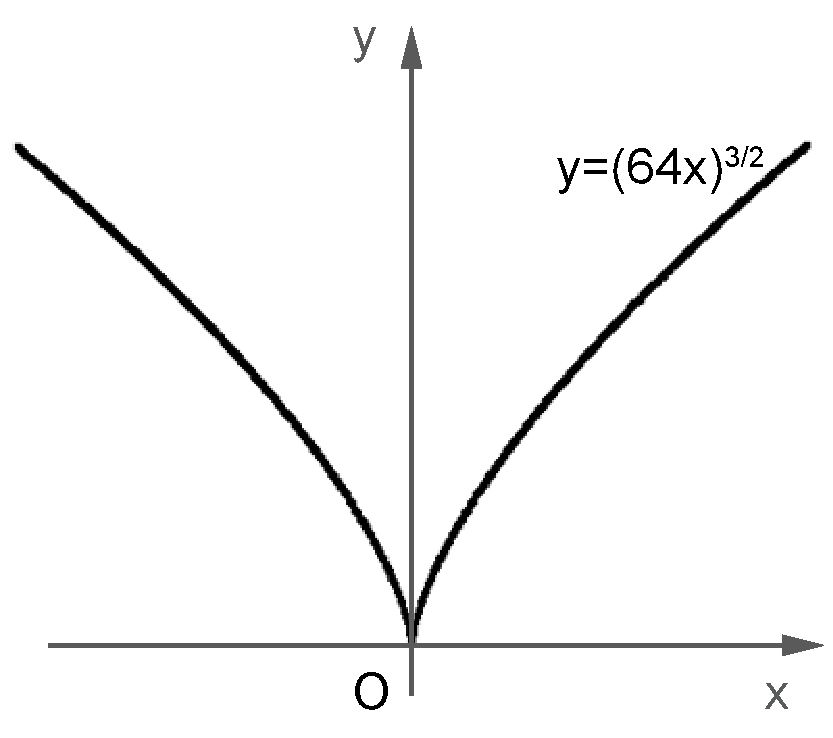
\includegraphics[width=0.4\textwidth]{Mid2Curve.pdf}
      \caption{\small{The constraint $64x^2-y^3=0$.}}
  \end{center}
\end{figure}
\item Setting $\nabla f = \lambda \nabla g$ yields the equations
\begin{align}
  0 &=128 \lambda x , \\
  1 &=-3\lambda y^2 . \label{utfdjtcw45f}
\end{align}
The first equation is satisfied if $\lambda=0$ or if $x=0$. But the second equation gives us that $\lambda \ne 0$, so $x$ must be equal to 0 (which is true). Substituting $x=0$ into the constraint $64x^2-y^3=0$ yields $y=0$, which, indeed, is the $y$-coordinate of the minimum value that we found in part (a). However, substitution of $y=0$ into Equation (\ref{utfdjtcw45f}) yields an inconsistent result: $1 = -3\lambda (0)^2$, or $1=0$. 
\EEN
% ~~~~~~~~~~~~~~~~~~~~~~~~~~~~~~~~~~~~~~~~~~~~~~~~~~~~~~~~~~~~~~~~~~~~~~~~~~~~~~~~~
\item % SIMPLE CHAIN RULE
Applying the chain rule yields
\begin{align*}
  \frac{d}{dt}g(t)
  &=\frac{d}{dt} f(\sin t, e^t+\cos t) \\
  &= \frac{\partial f}{\partial x}\cdot\frac{d \sin t}{d t} +  \frac{\partial f}{\partial y}\cdot\frac{d (e^t \cos t)}{d t} \\
  &= \cos t\frac{\partial f}{\partial x} +  (e^t - \sin t) \frac{\partial f}{\partial y}
\end{align*}
% ~~~~~~~~~~~~~~~~~~~~~~~~~~~~~~~~~~~~~~~~~~~~~~~~~~~~~~~~~~~~~~~~~~~~~~~~~~~~~~~~~
\item % WAVE EQUATION
Applying the chain rule yields
\begin{align*}
  \ut &= f'(s-ct)\frac{\partial (s-ct)}{\partial t} + g'(s+ct)\frac{\partial (s+ct)}{\partial t} \\ &= -c f'(s-ct) + cg'(s+ct).
\end{align*}
Differentiating again yields
\begin{align*}
  \utt &= ( -c)^2 f''(s-ct) + c^2g''(s+ct) \\& =  c^2 f''(s-ct) + c^2g''(s+ct)
\end{align*}
Similarly:
\begin{align*}
  \us &= f'(s-ct)\frac{\partial (s-ct)}{\partial s} + g'(s+ct)\frac{\partial (s+ct)}{\partial s} \\& = f'(s-ct) + g'(s+ct) \\
  \uss &= f''(s-ct) + g''(s+ct) 
\end{align*}
By comparison, \begin{align*}\utt = c^2\uss \end{align*}.
% ~~~~~~~~~~~~~~~~~~~~~~~~~~~~~~~~~~~~~~~~~~~~~~~~~~~~~~~~~~~~~~~~~~~~~~~~~~~~~~~~~
\item % CYLINDERS VOLUME
Using cylindrical coordinates, $ z =\ln(x^2+y^2) = \ln(r^2)$, and $1 \le r^2 \le 4$, or $1\le r \le 2$. The desired volume is given by the triple integral
\begin{align*}
  {\int_0^{2\pi} \!\! \int_{1}^{2} \!\! \int_{0}^{\ln r^2}} r\ dz dr d\theta 
  &= {\int_0^{2\pi} \!\! \int_{1}^{2}} r\ln r^2 \  dr d\theta \\
  &=2\pi \int_{1}^{2} r\ln r^2 \  dr 
\end{align*}
Let $u=r^2$, then $du = 2rdr$, and our integral becomes
\begin{align*}
  {\int_0^{2\pi} \!\! \int_{1}^{2} \!\! \int_{0}^{\ln r^2}} r\ dz dr d\theta 
  &=2\pi \int_{1}^{2} r\ln r^2 \  dr \\
  &=2\pi \int_{1}^{4} \ln u \  du  \\
  &=2\pi\Big( u \ln u -u \Big)\Big|_{1}^{4}  \\
  &=2\pi\Big( (4 \ln 4 -4)-(\ln 1 -1)  \Big)  \\
  &=2\pi (4 \ln 4 - 3)
\end{align*}
% ~~~~~~~~~~~~~~~~~~~~~~~~~~~~~~~~~~~~~~~~~~~~~~~~~~~~~~~~~~~~~~~~~~~~~~~~~~~~~~~~~
\item % FUNCTION THAT IS NOT A GRADIENT
\BEN
\item Let $f(x,y) = y \MB{i} + y \MB{j}$. This function has the property that there does not exist an $F(x,y)$ such that $\nabla F = f(x,y)$. 
\item If $\nabla F = f$, then 
\begin{align}
  \frac{\partial F}{\partial x} &= g_1 = y \\
  \frac{\partial F}{\partial y} &= g_2 = y 
\end{align}
But the first equation implies that $F=xy+\phi(y)$, where $\phi$ is an arbitrary function of $y$. Differentiating with respect to $y$ gives us
\begin{align}
  \frac{\partial F}{\partial y} &= \py \Big(xy+\phi(y)\Big) = x + \phi'(y)
\end{align}
There does not exist a $\phi'(y)$ such that this is equal to $g_2=y$. Therefore, the function we chose in part (a) is not a gradient of a function. 
\EEN
% ~~~~~~~~~~~~~~~~~~~~~~~~~~~~~~~~~~~~~~~~~~~~~~~~~~~~~~~~~~~~~~~~~~~~~~~~~~~~~~~~~

\end{enumerate}

\end{document}
